\subsection{Import ASTERIX Recording}
\label{sec:ui_import_asterix}

This task allows importing of ASTERIX data recording files into the opened database. \\

\begin{figure}[H]
  \center
    \hspace*{-0.5cm}
    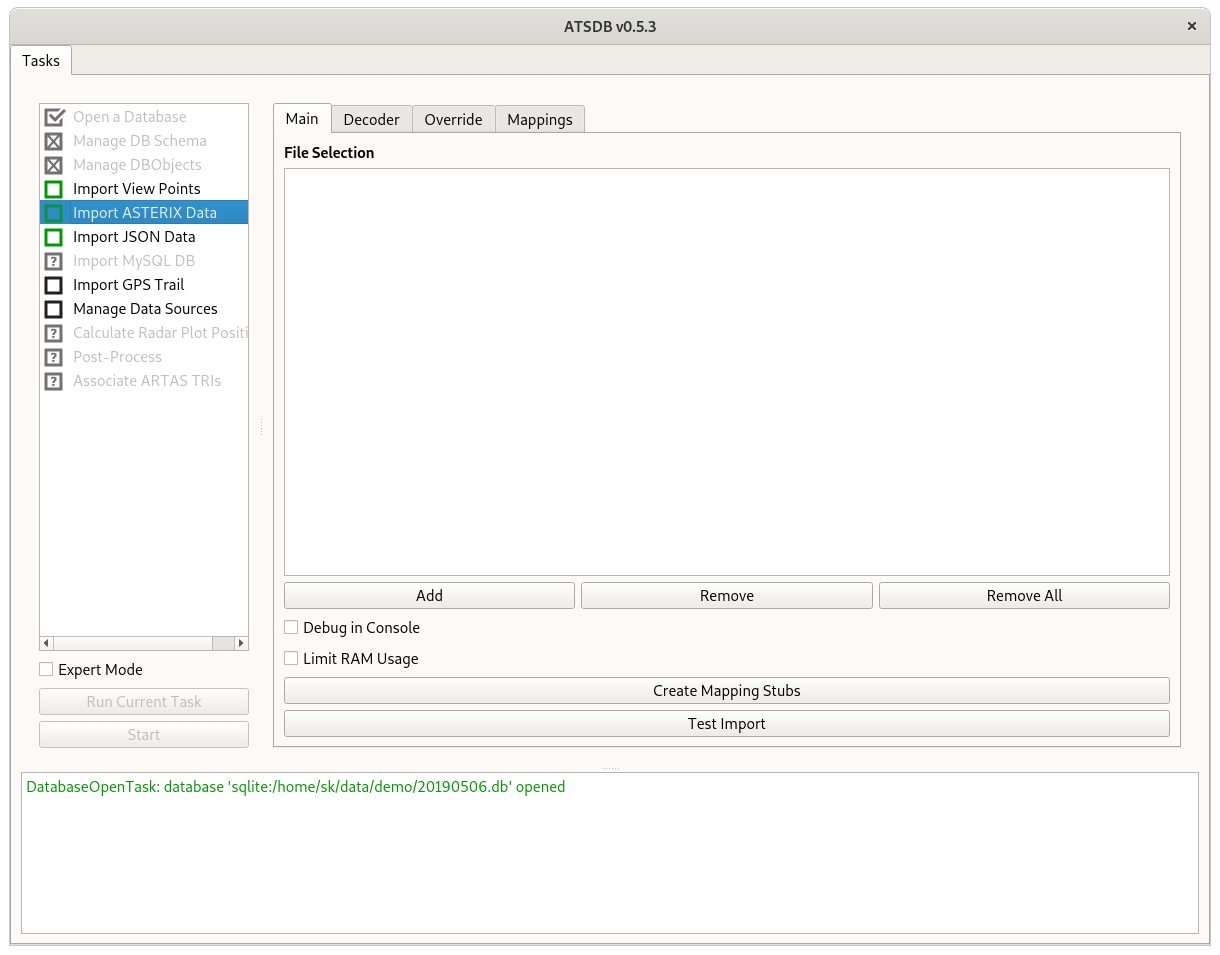
\includegraphics[width=17cm]{figures/asterix_import_data.png}
  \caption{Import ASTERIX data}
\end{figure}

There exist 3 tabs:

\begin{itemize}
\item Main: File label, input line, jASTERIX decoder settings
\item Override: Data override settings
\item Mappings: Definition of created database content based on decoded data
\end{itemize}
\ \\

Please note that the following framings are currently supported:
\begin{itemize}
\item None: Raw, netto, unframed ASTERIX data blocks
\item IOSS: IOSS Final Format
\item IOSS\_SEQ: IOSS Final Format with sequence numbers
\item RFF: Comsoft RFF format
\end{itemize}
\ \\

Please note that the following ASTERIX categories, editions, reserved expansion fields and special purpose fields are currently supported: \\

\begin{tabular}{ | l | r | r | r |}
\hline
  CAT & Editions & REFs & SPFs  \\ \hline
  001 & 1.1 &  &  \\ \hline
  002 & 1.0 &  &  \\ \hline
  010 & 0.24 Sensis, 0.31  &  &  \\ \hline
  019 & 1.2, 1.3 & & \\ \hline
  020 & 1.5, 1.8 & 1.3 & \\ \hline
  021 & 2.1, 2.4 & & \\ \hline
  023 & 1.2 & & \\ \hline
  034 & 1.26 & & \\ \hline
  048 & 1.15, 1.23 & 1.9 & \\ \hline
  062 & 1.12, 1.16, 1.18 & 1.2 & ARTAS TRIs \\ \hline
  063 & 1.0, 1.1 & & \\ \hline
  065 & 1.2, 1.3 & & \\ \hline
\end{tabular} \\
\  \\

Please note that sensor status messages can be decoded, but are not inserted into the database. Decoding of ASTERIX CAT002 is recommended if CAT001 data is imported, since the timestamps are derived from it (if not available in CAT001).

\subsection{Main Tab}

At the top, the recording file to be imported is shown. Below, there exists a combobox defining in which line the data should be written. \\

\paragraph{Framing}
Using the 'Framing' drop-down menu, the current framing can be selected. Using the 'Edit' button, the current framing definition is opened in a text editor.

\paragraph{Categories}

For each category, a number of elements exist:

\begin{itemize}
\item Category checkbox: Number of category and checkbox defining if it should be decoded
\item Edition: Drop-down menu to select the edition number to be used
\item Edition Edit Button \includegraphics[width=0.5cm]{../../data/icons/edit.png}: Opens the current edition definition in a text editor
\item REF: Drop-down menu to select the Reserved Expansion Field defition (if available)
\item REF Edit Button \includegraphics[width=0.5cm]{../../data/icons/edit.png}: Opens the current REF definition in a text editor
\item SPF: Drop-down menu to select the Special Purpose Field defition (if available)
\item SPF Edit Button \includegraphics[width=0.5cm]{../../data/icons/edit.png}: Opens the current SPF definition in a text editor
\end{itemize}
\ \\

\paragraph{Additional}

Using the 'Edit Data Block' button, the ASTERIX data block definition is opened in a text editor. \\

Using the 'Edit Categories' button, the ASTERIX definitions file is opened in a text editor. \\

Using the 'Refresh' button, the all of the jASTERIX definitions are re-loaded from the harddisk (e.g. to update after file changes were made). \\



\paragraph{Running}
Using the 'Debug in Console' checkbox, additional debugging information is output to the console, and the ASTERIX decoding is switched to single-threading for easier investigation. \\

The 'Cancel' button aborts the import, using the 'Test Import' button the import function can be tested without inserting the data into the database, the 'Import' imports the selected file with the given options. This function can be run multiple times. \\


\subsection{Override Tab}
\label{sec:task_import_asterix_override}


\begin{figure}[H]
  \center
    \hspace*{-0.5cm}
    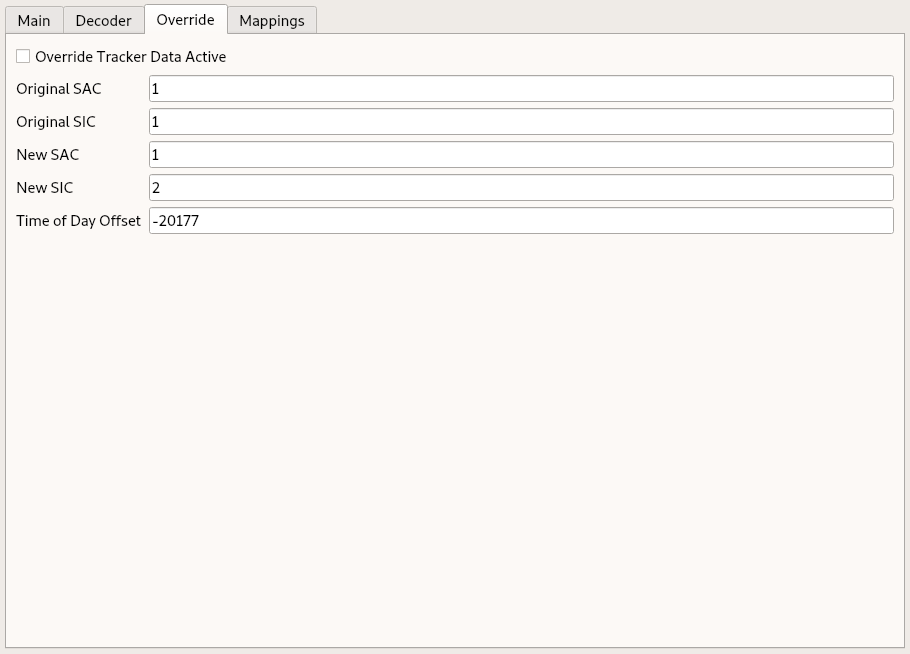
\includegraphics[width=17cm]{figures/asterix_import_data_override.png}
  \caption{Task: Import ASTERIX data override}
\end{figure}

This feature should only be used in very specific circumstances. When activated, the function adds a Time of Day offset to all imported data, to compensate time offsets (e.g. when importing data from a replay). \\

\begin{itemize}
\item 'Override Time of Day Active' checkbox: When the override is active. Disabled by default.
\item Time of Day Offset: Positive or negative offset to be added, in seconds. If the resulting value is out of bounds, it is adjusted to the [0, 86400] interval.
\end{itemize}
\ \\

\subsection{Mappings Tab}

\begin{figure}[H]
  \center
    \hspace*{-0.5cm}
    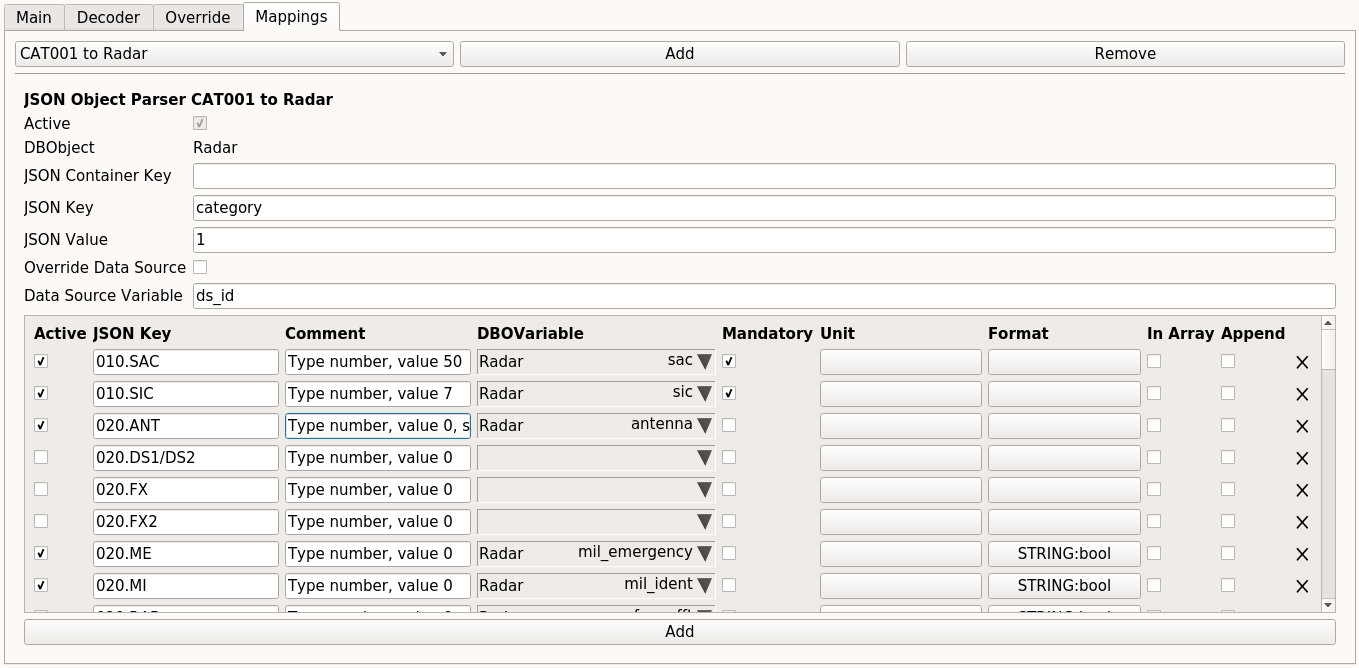
\includegraphics[width=17cm]{figures/asterix_import_data_mappings.png}
  \caption{Task: Import ASTERIX Data Mappings}
\end{figure}

At the top, the GUI elements can be used to show/add/remove ASTERIX JSON parsers. Below that, the currently selected ASTERIX JSON parser is shown and can be configured. \\

An ASTERIX JSON parser in this context is the function that parses the JSON content created by the jASTERIX parser, and creates database content from it. For each category a dedicated parser defines the mapping from JSON to database content. \\

For common users normally no interaction is recommended, but it might be sometimes interesting what database content is created from which ASTERIX data.

\paragraph{Top Elements}

Using the drop-down menu, the to-be-shown parser can be selected. The buttons allow for adding and removing ASTERIX JSON object parsers.

\paragraph{Parser GUI Elements}

The exact definition of how the parsing works is out of scope for this document, so only a short summy is given here. For more information please contact the author.

In the mappings list, the following columns are given:

\begin{itemize}
\item Active checkbox: Defines if the specific mapping is used
\item JSON Key: JSON location and name of the data to be mapped, commonly in 'Data Item Number'.'variable' or 'Data Item Number'.'Sub Item'.'variable' format
\item DBContent Variable: Target variable to which this data is mapped
\end{itemize}
\ \\

Whenever a mapping is selected, the details are shown on the right hand side, giving details about the ASTERIX information (based on the jASTERIX specifications) and the DBContent variable it is mapped to. Using the 'Show DBContent Variable' button the variable can be inspected in detail.

\begin{figure}[H]
  \center
    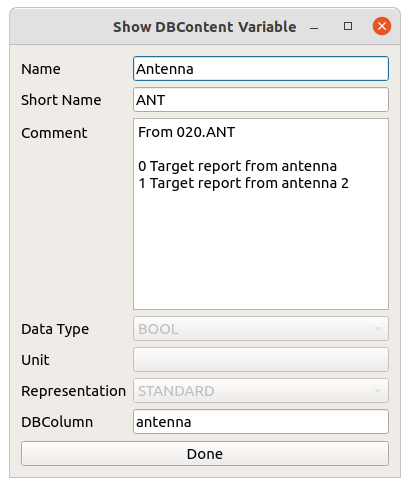
\includegraphics[width=7cm]{figures/asterix_import_data_dbcont_var_details.png}
  \caption{Task: Import ASTERIX Data DBContent Variable Details}
\end{figure}

\subsection{Running}

Using the 'Import' button the task can be performed. During import a status indication will be shown. \\

\begin{figure}[H]
  \center
    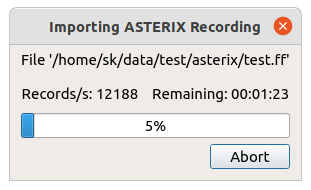
\includegraphics[width=5cm]{figures/asterix_import_data_status.png}
  \caption{Import ASTERIX Data Status}
\end{figure}

If an decoding error occurs, a brief message box is shown, after which the application has to be closed. Please make sure that the correct framing and edition versions are selected, or contact the author for support if this does not resolve the issue. \\


\paragraph{Comments}
Importing performance strongly depends on CPU performance (multi-threading very beneficial), but a import of 5 million target reports takes about 3:30 minutes on the author's hardware. \\

The (truncated) timestamps of CAT001 are calculated in a simple algorithm based on the CAT002 messages from the same sensor, so their timestamp data is slightly unreliable, but exact enough for e.g. time window filtering. \\

This task can be run several times, e.g. if multiple ASTERIX recordings from different data sources are to be imported. \\

\includegraphics[width=0.5cm]{../../data/icons/hint.png} Please note the currently not all data fields (as shown in the JSON object parsers) are imported.\\


